\chapter{测试装置的基本特性}
\label{chap:measurement-systems}

\begin{focusbox}{本章复习路线}
第2章回答“信号由哪些频率组成”，本章进一步回答“这些成分通过测试装置后如何改变”。先用静态标定确定输入与输出的比例，再用动态模型计算每个频率的幅值比和相位差。本章的知识主线是：
\[
\text{静态指标}\ \longrightarrow\ H(s),\ H(\iu\omega),\ h(t)
\ \longrightarrow\ \text{一阶与二阶响应}\ \longrightarrow\ \text{不失真测试}.
\]
\textbf{学习目标：}能区分静态特性指标，建立和使用一阶、二阶模型，计算多频信号的稳态输出，并依据误差要求选择时间常数、固有频率和阻尼比。
\end{focusbox}

\begin{table}[H]
\centering\small
\begin{tabularx}{\linewidth}{@{}p{3.4cm} X@{}}
\toprule
复习模块 & 核心能力 \\
\midrule
静态标定与指标 & 区分灵敏度、线性度、回程误差、分辨力与重复性。 \\
动态模型 & 明确零初始条件，联系微分方程、传递函数、频响与冲激响应。 \\
一阶装置 & 用 $\omega\tau$ 判断幅值衰减、相位滞后和可用频带。 \\
二阶装置 & 用 $r=\omega/\omega_n$、$\zeta$ 判断共振、幅相变化及阻尼选择。 \\
不失真测试 & 检查幅频平坦与相频线性，区分波形要求与幅值误差要求。 \\
典型例题 & 分频计算稳态响应，由允许误差反求参数，并解释计算结果。 \\
\bottomrule
\end{tabularx}
\end{table}

\section{概述：测试装置作为信号转换系统}

\subsection{静态标定、标准传递与测量链}

测试装置将被测输入 $x(t)$ 转换为可观察的输出 $y(t)$。测量链通常包含传感器、信号调理与显示记录环节；每个环节都可能改变信号，也可能引入误差。

\dfn{静态标定}{在其余影响量保持不变的条件下，逐点改变被测输入，待输出稳定后记录输入与输出，得到静态特性曲线。标定时还应安排正、反行程与同方向重复测量，以识别回程误差和重复性。}

\textbf{标准传递：}通过参考标准、工作标准及实际仪器之间的逐级比较，把统一的量值传递到测量现场。标定曲线给出装置的输入输出关系，量值溯源则说明这个关系依据何种标准建立。

\textbf{静态特性}描述恒定或缓慢变化输入下的关系；\textbf{动态特性}描述快速变化输入下的响应。静态标定准确，并不保证装置能准确跟随快速信号。

\subsection{线性、时不变、因果与动态系统}

\dfn{线性与时不变}{若 $x_1(t)\to y_1(t)$、$x_2(t)\to y_2(t)$，线性要求
\[
c_1x_1(t)+c_2x_2(t)\ \longrightarrow\ c_1y_1(t)+c_2y_2(t).
\]
其中包含叠加性与比例性。时不变要求：若 $x(t)\to y(t)$，则任意时间平移后的 $x(t-t_0)\to y(t-t_0)$。本章主要研究\textbf{线性时不变系统}，简称LTI系统。}

\begin{itemize}
\item \textbf{因果系统：}当前输出只取决于当前与过去的输入，冲激响应满足 $h(t)=0$（$t<0$）。
\item \textbf{无记忆系统：}输出仅取决于同一时刻的输入，如理想比例环节 $y(t)=Kx(t)$。
\item \textbf{动态系统：}包含储能、惯性或记忆，响应需要一定时间建立，如电容充电、质量块振动。
\item \textbf{集总参数与分布参数：}前者用有限个集中元件建模，常得到常微分方程；后者还需考虑空间分布。
\end{itemize}

\thm{线性时不变装置的频率保持性}{对稳定LTI系统，正弦输入的稳态输出仍为\textbf{同频率}正弦信号，改变的是幅值与相位。多频输入可按叠加原理逐频计算，再相加得到稳态输出。}

\nt{频率保持性还需要时不变条件；仅有线性并不足够。例如 $y(t)=\cos\omega_ct\,x(t)$ 对输入是线性的，但会搬移频谱。装置也只有在其线性工作范围内才适用本章模型；饱和、间隙及明显非线性可能引入新的频率成分。}

\subsection{系统分析的三类问题与实际要求}

\begin{table}[H]
\centering
\begin{tabularx}{\linewidth}{@{}l l X@{}}
\toprule
问题 & 已知量 & 求解与用途 \\
\midrule
系统辨识 & 输入、输出 & 求系统特性；据此标定或选用仪器。 \\
输入反求 & 系统、输出 & 推断被测输入；衰减与噪声会影响反求精度。 \\
响应预测 & 输入、系统 & 计算输出，分析装置对信号幅值、相位与波形的影响。 \\
\bottomrule
\end{tabularx}
\end{table}

\textbf{负载效应：}测量装置接入后可能改变被测对象，如电压表输入电阻有限会改变原电路电压；前后级连接也可能因阻抗不匹配改变传输特性。\textbf{抗干扰性：}需考虑电源、环境电磁场、声光温度、振动与信道噪声。选择装置时，静态精度、动态带宽、负载效应和抗干扰能力应一起考虑。

\clearpage
\section{测试装置的静态特性}

\subsection{理想直线、灵敏度与量程}
\noindent\keypoint{复习重点：灵敏度有量纲，是输入输出曲线的斜率；灵敏度高不等于测量准确。}

\dfn{静态灵敏度}{理想线性标定关系可写为
\[
y=y_0+Sx,\qquad S=\frac{\Delta y}{\Delta x}.
\]
对非线性曲线，局部灵敏度为 $S(x)=\diff y/\diff x$。$S$ 的单位为“输出单位/输入单位”；仅当输入、输出同量纲时，才可视为无量纲放大倍数。}

当零点偏置 $y_0$ 已扣除时，理想关系为 $y=Sx$。若输出可用范围固定，增大灵敏度会减小相应的输入量程，也可能使噪声、漂移与过载更显著。因此应依据最小待测变化和最大输入选择灵敏度。

\ex{由输出分辨力估算输入分辨力}{若位移传感器灵敏度为 $S=300\,\mathrm{mV/mm}$，显示环节可分辨的输出变化为 $3\,\mathrm{mV}$，在噪声和漂移可忽略时，输入分辨力约为
\[
\Delta x_{\min}\approx\frac{\Delta y_{\min}}{|S|}
=\frac{3}{300}\,\mathrm{mm}=0.01\,\mathrm{mm}.
\]
该结果是分辨力估计，并未包括标定误差、迟滞和其他准确度限制。}

\subsection{线性度、回程误差、分辨力与重复性}

\dfn{线性度与回程误差}{记输出满量程跨度 $Y_{\mathrm{FS}}=Y_{\max}-Y_{\min}>0$。
相对规定参考直线的最大输出偏差为 $\Delta_{\max}$，线性误差指标为
\[
e_L=\frac{\Delta_{\max}}{Y_{\mathrm{FS}}}\times100\%.
\]
同一输入下正、反行程输出最大差值为 $h_{\max}$，回程误差为
\[
e_H=\frac{h_{\max}}{Y_{\mathrm{FS}}}\times100\%.
\]
参考直线可按端点连线或最小二乘拟合确定；方法不同，线性度数值也可能不同，报告时需注明。}

回程误差也称迟滞或迟环，说明输出还与输入变化方向或历史有关。机械间隙、摩擦、磁性材料磁滞及材料内摩擦等均可能造成迟滞。

\dfn{分辨力与重复性}{分辨力是能使输出产生可察觉变化的\textbf{最小输入变化量}。重复性考察相同条件下、输入沿\textbf{同一方向}多次全量程测量时，输出特性的一致程度。若采用最大曲线间差值 $B_{\max}$ 的约定，则
\[
e_R=\frac{B_{\max}}{Y_{\mathrm{FS}}}\times100\%.
\]
不同统计定义下的重复性指标需按相应规定计算。}

\begin{center}
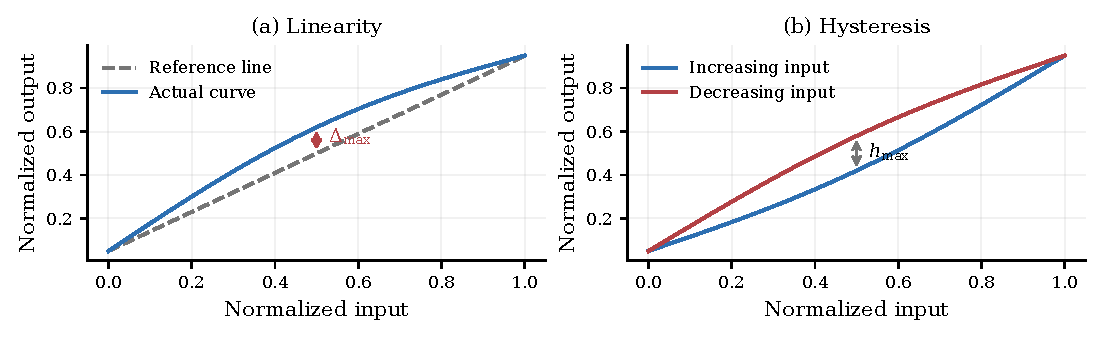
\includegraphics[width=.98\linewidth]{ch3-static-characteristics.pdf}
\end{center}
图中为归一化示意：左图比较实际曲线与参考直线，右图比较同一输入的正、反行程输出。两种偏差的比较对象不同。

\begin{table}[H]
\centering\small
\begin{tabularx}{\linewidth}{@{}p{2.3cm} X X@{}}
\toprule
指标 & 主要回答的问题 & 判断时的比较对象 \\
\midrule
灵敏度 & 输入变化能产生多大输出变化？ & 输出增量与输入增量之比。 \\
线性度 & 曲线偏离参考直线多少？ & 实测曲线与规定直线。 \\
回程误差 & 输入方向改变会影响输出吗？ & 同一输入的正、反行程。 \\
分辨力 & 多小的输入变化能被察觉？ & 最小可察觉输入变化。 \\
重复性 & 重复测量是否一致？ & 同条件、同方向的多次曲线。 \\
\bottomrule
\end{tabularx}
\end{table}

\nt{以上相对误差通常以\textbf{满量程输出跨度}为分母，不能随意换成某个读数。高灵敏度、高分辨力与高准确度是不同概念；重复性好也可能同时存在稳定的系统偏差。}

\clearpage
\section{动态特性的三种数学描述}

\subsection{从微分方程到传递函数}
\noindent\keypoint{复习重点：传递函数表示零初始条件下的输入输出关系，不能遗漏初始状态的影响。}

对可用常系数线性微分方程建模的装置，写成
\[
\sum_{k=0}^{n}a_k\frac{\diff^ky(t)}{\diff t^k}
=\sum_{k=0}^{m}b_k\frac{\diff^kx(t)}{\diff t^k}.
\]
这里 $\diff^0y/\diff t^0=y$，各系数由装置参数和输入输出变量决定。

\dfn{传递函数}{采用单边拉普拉斯变换
\[
X(s)=\int_{0^-}^{\infty}x(t)e^{-st}\diff t,\qquad s=\sigma+\iu\omega.
\]
零初始条件下，微分对应乘 $s$，从而
\[
\boxed{H(s)=\frac{Y(s)}{X(s)}
=\frac{b_ms^m+\cdots+b_1s+b_0}{a_ns^n+\cdots+a_1s+a_0}}.
\]
传递函数由系统及选定的输入输出关系决定，与具体输入波形无关。}

一般有 $\mathcal L\{y'(t)\}=sY(s)-y(0^-)$。初始状态不为零时，总输出包含\textbf{零输入响应}与\textbf{零状态响应}；$Y(s)=H(s)X(s)$ 单独描述后者。

\textbf{极点与零点：}约分后分母根为极点，分子根为零点。极点决定自然响应的模式，零点也会影响幅相特性；两者均与模型参数、输入输出位置有关。$H(s)$ 的单位为输出单位除以输入单位，静态增益在适用时为 $H(0)$。

\nt{“分母阶数高于分子阶数”不等于稳定。对约分后的因果有理传递函数，BIBO稳定要求所有极点位于左半平面。例如 $1/(s-1)$ 严格真有理却不稳定，比例环节 $H(s)=K$ 没有惯性但可稳定。判断稳定性应检查极点，不能只比较阶数。}

\subsection{频率响应、幅频与相频特性}

\dfn{频率响应函数}{对稳定LTI系统，在虚轴上令 $s=\iu\omega$，得到
\[
H(\iu\omega)=P(\omega)+\iu Q(\omega)
=A(\omega)e^{\iu\phi(\omega)},
\]
\[
A(\omega)=|H(\iu\omega)|=\sqrt{P^2+Q^2},\qquad
\phi(\omega)=\operatorname{atan2}(Q,P).
\]
$A$ 为输出与输入的幅值比，$\phi$ 为\textbf{输出相位减去输入相位}。}

对 $x(t)=X_0\cos(\omega t+\theta)$，$X_0\geq0$，稳态输出为
\[
\boxed{y_{\mathrm{ss}}(t)=X_0A(\omega)
\cos\bigl[\omega t+\theta+\phi(\omega)\bigr]}.
\]
输入为正弦时也按同一规则处理。装置不改变正弦的频率；原输入相位 $\theta$ 必须保留，再加上系统相位差。

\textbf{与第2章的联系：}若沿用 $f$ 为Hz的傅里叶变换约定，则
\[
Y(f)=H(\iu2\pi f)X(f),\qquad \omega=2\pi f.
\]
这里 $X(f)$ 是输入频谱，$H(\iu2\pi f)$ 是装置频响，两者含义与量纲不同。

幅频与相频曲线分别画 $A$、$\phi$ 随频率的变化；奈奎斯特图在复平面画 $Q$ 对 $P$ 的轨迹；伯德图以对数频率为横轴，画对数幅值与相位。若 $H$ 有量纲，可先除以参考增益，如画 $20\log_{10}[A(\omega)/K]$。

\subsection{冲激响应、卷积与环节组合}

\dfn{单位冲激响应}{零初始条件下，输入 $\delta(t)$ 时的输出为 $h(t)$。因 $\mathcal L\{\delta(t)\}=1$，有
\[
h(t)=\mathcal L^{-1}\{H(s)\},\qquad
H(s)=\mathcal L\{h(t)\}.
\]
对稳定系统还可写
\[
H(\iu\omega)=\int_{-\infty}^{\infty}h(t)e^{-\iu\omega t}\diff t.
\]
因此，$h(t)$、$H(s)$ 与 $H(\iu\omega)$ 是同一系统在时域、复频域与频域的描述。}

\thm{零状态响应与串并联}{任意输入的零状态响应为
\[
y(t)=(h*x)(t)=\int_{-\infty}^{\infty}h(\lambda)x(t-\lambda)\diff\lambda.
\]
无额外负载相互作用时，串联环节的传递函数相乘，并联且输出相加时传递函数相加：
\[
H_{\mathrm{series}}(s)=\prod_{i=1}^{N}H_i(s),\qquad
H_{\mathrm{parallel}}(s)=\sum_{i=1}^{N}H_i(s).
\]
串联的幅值比相乘、相位相加；并联须\textbf{先做复数相加}，再求模和相角。}

在适用的光滑性与零状态条件下，LTI卷积还给出 $x'(t)\to y'(t)$；输入积分也对应输出积分。若直接从 $t=0$ 积分，要核对边界值与初始条件，不能任意丢弃常数项。

\clearpage
\section{一阶测试装置的特性与时间常数}

\subsection{标准模型与物理意义}
\noindent\keypoint{复习重点：先识别 $K$ 与 $\tau$，再用无量纲变量 $q=\omega\tau$ 计算动态变化。}

\dfn{一阶惯性环节}{对
\[
a_1y'(t)+a_0y(t)=b_0x(t),
\]
令 $\tau=a_1/a_0>0$、$K=b_0/a_0$，可得
\[
\tau y'(t)+y(t)=Kx(t),\qquad
\boxed{H(s)=\frac{K}{1+\tau s}}.
\]
$K$ 是静态灵敏度，$\tau$ 是时间常数，单位为秒。以下幅相公式取 $K>0$；归一化增益时令 $K=1$。}

RC低通电路以电容电压为输出时，$K=1$、$\tau=RC$。机械黏性阻尼与弹簧构成的一阶近似系统有 $c y'+ky=F$，则 $K=1/k$、$\tau=c/k$。物理系统不同，可以具有相同形式的传递函数。

\subsection{幅值衰减、相位滞后与转折频率}

\thm{一阶频率响应}{令 $q=\omega\tau\geq0$，则
\[
H(\iu\omega)=\frac{K}{1+\iu q},\qquad
\boxed{\frac{A(\omega)}{K}=\frac{1}{\sqrt{1+q^2}}},\qquad
\boxed{\phi(\omega)=-\arctan q}.
\]
当 $q\ll1$ 时，$A/K\approx1-q^2/2$，$\phi\approx-q=-\omega\tau$；低频范围近似为比例放大并延迟 $\tau$。}

\begin{center}
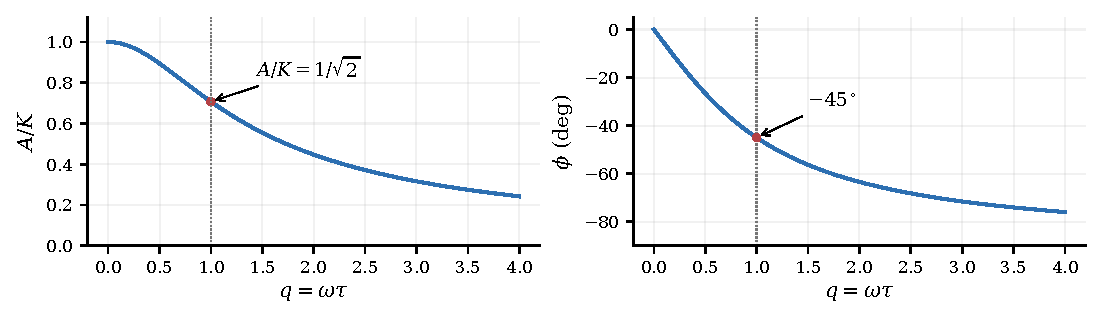
\includegraphics[width=.98\linewidth]{ch3-first-order-frequency.pdf}
\end{center}
横轴 $q=\omega\tau$；右图用角度表示相位，曲线的低频近似公式采用弧度。

\begin{table}[H]
\centering
\begin{tabular}{@{}c c c l@{}}
\toprule
$q$ & $A/K$ & $\phi$ & 含义 \\
\midrule
$0$ & $1$ & $0$ & 静态输入不衰减（归一化后）。 \\
$0.2$ & $0.9806$ & $-11.31^\circ$ & 幅值误差约 $1.94\%$。 \\
$1$ & $1/\sqrt2$ & $-45^\circ$ & 转折频率，归一化幅值为 $-3.01\,\mathrm{dB}$。 \\
$q\to\infty$ & $0$ & $-90^\circ$ & 高频成分衰减显著。 \\
\bottomrule
\end{tabular}
\end{table}

转折角频率和转折频率分别为
\[
\omega_c=\frac{1}{\tau},\qquad f_c=\frac{1}{2\pi\tau}.
\]
高频时 $A/K\sim1/q$，伯德幅频渐近斜率为 $-20\,\mathrm{dB/dec}$。\textbf{幅值误差只有几个百分点的测量频带，应比 $f_c$ 小得多。}

\subsection{阶跃与冲激响应：怎样理解 $\tau$}

对阶跃输入 $x(t)=X_0u(t)$ 且 $y(0^-)=0$，解一阶方程得
\[
\boxed{y(t)=KX_0(1-e^{-t/\tau})u(t)},\qquad
\boxed{h(t)=\frac{K}{\tau}e^{-t/\tau}u(t)}.
\]
阶跃响应单调趋于 $KX_0$，无超调。$t=\tau$ 时达到终值的 $1-e^{-1}\approx63.2\%$；$3\tau$ 时约为 $95.0\%$，$4\tau$ 时约为 $98.2\%$。

\begin{center}
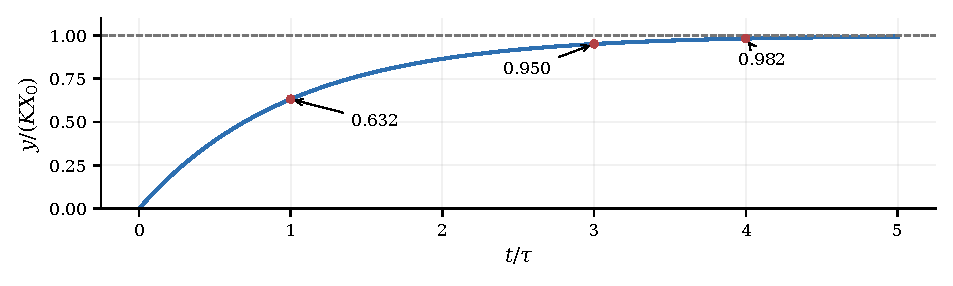
\includegraphics[width=.85\linewidth]{ch3-first-order-step.pdf}
\end{center}

若剩余相对误差要求为 $\varepsilon$，则 $e^{-t/\tau}\leq\varepsilon$，所需时间满足 $t\geq-\tau\ln\varepsilon$。因此 $\tau$ 越小，响应越快，给定幅值误差下可测频率越高。

\subsection{由允许振幅误差反求时间常数}

以静态标定后的理想幅值为基准，定义\textbf{振幅误差的大小}
\[
e_A=\left|\frac{A(\omega)}{K}-1\right|.
\]
一阶低通只衰减，因此 $e_A=1-1/\sqrt{1+(\omega\tau)^2}$。给定 $0<\varepsilon<1$，由 $e_A\leq\varepsilon$ 得
\[
\frac{1}{\sqrt{1+(\omega\tau)^2}}\geq1-\varepsilon
\quad\Longrightarrow\quad
\boxed{\tau\leq\frac{\sqrt{(1-\varepsilon)^{-2}-1}}{\omega}}.
\]
若要求整个 $0\leq f\leq f_m$ 频带均满足误差，只需在最高频率 $\omega_m=2\pi f_m$ 检查，因为一阶幅值随频率单调下降。

\nt{时间常数的设计结果是\textbf{上限}，并非唯一数值。取等号得到边界设计，更小的 $\tau$ 也合格。幅值误差小并不意味着相位差为零；相位要求需另行检查。}

\clearpage
\section{二阶测试装置的特性与阻尼比}

\subsection{标准模型、固有频率与归一化}
\noindent\keypoint{复习重点：把实际频率化为 $r=\omega/\omega_n=f/f_n$，用双参数反正切保留相位象限。}

\dfn{二阶低通模型}{对 $a_2y''+a_1y'+a_0y=b_0x$，令
\[
K=\frac{b_0}{a_0},\qquad \omega_n=\sqrt{\frac{a_0}{a_2}},\qquad
\zeta=\frac{a_1}{2\sqrt{a_0a_2}},
\]
可写成
\[
\frac{1}{\omega_n^2}y''+\frac{2\zeta}{\omega_n}y'+y=Kx,
\qquad
\boxed{H(s)=\frac{K\omega_n^2}{s^2+2\zeta\omega_ns+\omega_n^2}}.
\]
$\omega_n$ 是无阻尼固有角频率，$f_n=\omega_n/(2\pi)$ 为固有频率，$\zeta$ 为无量纲阻尼比。以下取 $K>0$、$\omega_n>0$、$\zeta>0$。}

对质量、弹簧、阻尼系统 $m y''+c y'+ky=F(t)$，以位移为输出、力为输入，
\[
\omega_n=\sqrt{\frac{k}{m}},\qquad
\zeta=\frac{c}{2\sqrt{mk}},\qquad K=\frac{1}{k}.
\]
在位移式力测量中，可令标定后的输出 $z=ky$，使 $z/F$ 的静态增益归一化为1。增大刚度 $k$ 可提高固有频率，但同时减小位移灵敏度 $1/k$；带宽与灵敏度存在权衡。

\subsection{幅频、相频与三个关键位置}

\thm{二阶频率响应}{令 $r=\omega/\omega_n=f/f_n\geq0$，则
\[
H(\iu\omega)=\frac{K}{1-r^2+\iu2\zeta r},
\]
\[
\boxed{\frac{A(\omega)}{K}
=\frac{1}{\sqrt{(1-r^2)^2+(2\zeta r)^2}}},\qquad
\boxed{\phi(\omega)=-\operatorname{atan2}(2\zeta r,1-r^2)}.
\]
相位取从0连续下降到 $-\pi$ 的分支。}

\begin{center}
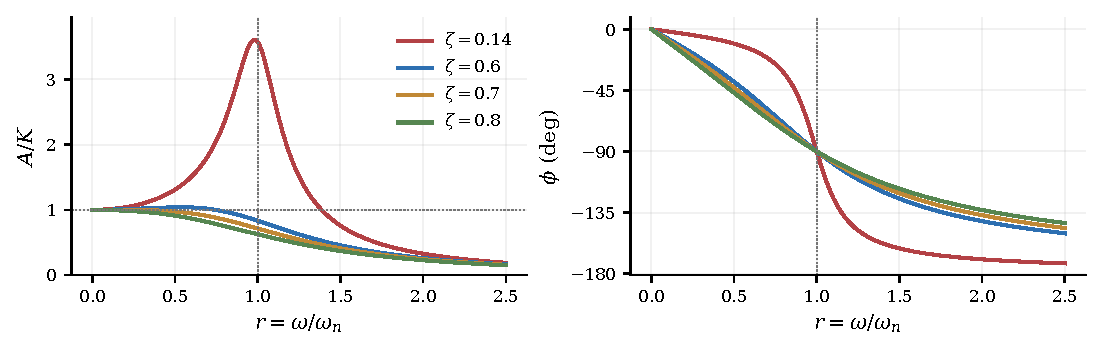
\includegraphics[width=.98\linewidth]{ch3-second-order-frequency.pdf}
\end{center}
图中归一化增益 $K=1$。小阻尼使固有频率附近出现强烈幅值放大；阻尼较大时幅频曲线更平缓，但低于固有频率的衰减也可能增大。

\begin{itemize}
\item $r\ll1$：$A/K\approx1+(1-2\zeta^2)r^2$，$\phi\approx-2\zeta r$，相位近似线性。
\item $r=1$：$A/K=1/(2\zeta)$，$\phi=-90^\circ$，适用于 $\zeta>0$。
\item $r\gg1$：$A/K\sim1/r^2\to0$，$\phi\to-180^\circ$；伯德幅频渐近斜率为 $-40\,\mathrm{dB/dec}$。
\end{itemize}

\nt{当 $r>1$ 时，分母实部 $1-r^2<0$，直接使用普通 $-\arctan[2\zeta r/(1-r^2)]$ 会丢失象限。应使用 $\operatorname{atan2}$ 或分段修正。高频端相位趋于 $-180^\circ$，但幅值趋于零，不能把高频曲线看似平缓理解为可作不失真测量。}

\subsection{欠阻尼与共振峰不是同一条件}

\begin{table}[H]
\centering
\begin{tabularx}{\linewidth}{@{}l l X@{}}
\toprule
阻尼比 & 自然响应类型 & 主要特点 \\
\midrule
$\zeta=0$ & 无阻尼 & 自由振动不衰减；固有频率处无有界正弦稳态响应。 \\
$0<\zeta<1$ & 欠阻尼 & 自然响应为衰减振荡，极点为共轭复数。 \\
$\zeta=1$ & 临界阻尼 & 不振荡，两个实极点重合。 \\
$\zeta>1$ & 过阻尼 & 不振荡，两个不同负实极点。 \\
\bottomrule
\end{tabularx}
\end{table}

判断\textbf{幅频曲线有无非零频率共振峰}，应求归一化幅值的最大值。令 $v=r^2\geq0$，分母平方为
\[
D(v)=(1-v)^2+4\zeta^2v
=v^2+(4\zeta^2-2)v+1.
\]
由 $D'(v)=2v+4\zeta^2-2$ 得
\[
\boxed{r_r=\sqrt{1-2\zeta^2},\quad
\frac{A_{\max}}{K}=\frac{1}{2\zeta\sqrt{1-\zeta^2}}}
\qquad\left(0<\zeta<\frac{1}{\sqrt2}\right).
\]
当 $\zeta\geq1/\sqrt2$ 时，幅值最大在 $r=0$，没有非零频率共振峰。因此 $1/\sqrt2\leq\zeta<1$ 仍是欠阻尼系统，却没有幅频共振峰。

\textbf{三个频率应分开：}无阻尼固有角频率 $\omega_n$；自由衰减振荡角频率 $\omega_d=\omega_n\sqrt{1-\zeta^2}$（欠阻尼）；幅频峰角频率 $\omega_r=\omega_n\sqrt{1-2\zeta^2}$（存在峰时）。它们通常不相等。

\subsection{阶跃、冲激响应与超调}

对欠阻尼情形 $0<\zeta<1$、零初始状态，单位冲激响应为
\[
h(t)=\frac{K\omega_n}{\sqrt{1-\zeta^2}}
e^{-\zeta\omega_nt}\sin(\omega_dt)u(t).
\]
对 $x(t)=X_0u(t)$，阶跃响应为
\[
\frac{y(t)}{KX_0}
=1-e^{-\zeta\omega_nt}
\left[\cos(\omega_dt)+\frac{\zeta}{\sqrt{1-\zeta^2}}\sin(\omega_dt)\right],
\quad t\geq0.
\]
其相对超调量为 $M_p=e^{-\pi\zeta/\sqrt{1-\zeta^2}}$，首次峰值时刻为 $t_p=\pi/\omega_d$。增大阻尼通常抑制振荡和超调，但过大的阻尼也可能使响应变慢。

\begin{center}
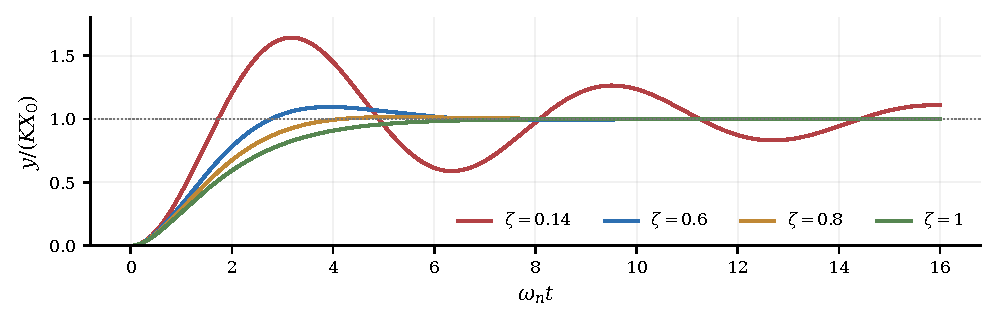
\includegraphics[width=.9\linewidth]{ch3-second-order-step.pdf}
\end{center}
图示各曲线终值均归一化为1；$\zeta=1$ 时阶跃响应为 $1-(1+\omega_nt)e^{-\omega_nt}$。这里的阶跃超调与正弦稳态共振峰是不同指标。

\subsection{为什么测量装置常取 $\zeta=0.6\sim0.8$}

\textbf{幅值方面：}小阻尼会放大固有频率附近的信号与干扰，增加过载风险。$\zeta$ 在 $0.6\sim0.8$ 附近可压低峰值，在一定低频范围保持接近静态增益。特别地，
\[
\left(\frac{A}{K}\right)^{-2}=1+(4\zeta^2-2)r^2+r^4.
\]
当 $\zeta=1/\sqrt2$ 时二次项消失，$A/K=1/\sqrt{1+r^4}$，低频幅频曲线较平坦。

\textbf{相位方面：}在 $r\ll1$ 时 $\phi\approx-2\zeta\omega/\omega_n$，可近似看作共同延迟 $t_0\approx2\zeta/\omega_n$。合理阻尼配合足够高的固有频率，有助于在可用频带内兼顾幅值平坦和相位近似线性。

\textbf{时间响应方面：}适度阻尼可减小过大的超调与长时间振铃。该区间是常用折中；具体选择仍需依据待测频带、幅值和相位误差要求，不能只凭阻尼比判断测量是否合格。

\clearpage
\section{实现不失真测试的条件}

\subsection{相同的比例与相同的时间延迟}
\noindent\keypoint{复习重点：多频信号要保持波形，要求各频率成分有相同幅值比例与相同时间延迟。}

\dfn{不失真测试}{若允许整体放大和整体延迟，理想输出为
\[
y(t)=A_0x(t-t_0),\qquad A_0>0,\quad t_0\geq0.
\]
利用第2章的时移性质，信号所占频带内必须满足
\[
\boxed{H(\iu\omega)=A_0e^{-\iu\omega t_0}},\qquad
\boxed{A(\omega)=A_0,\quad\phi(\omega)=-\omega t_0}.
\]
相位应按连续展开的分支理解，而不是要求主值相位图始终无跳变。}

\begin{center}
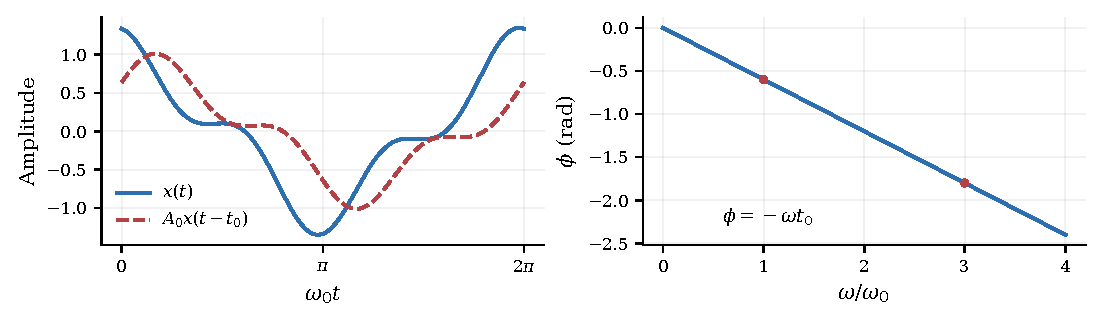
\includegraphics[width=.98\linewidth]{ch3-distortionless.pdf}
\end{center}
图示把两个谐波的幅值同乘 $A_0$，并施加同一延迟 $t_0$；延迟越高频率的成分，其相位变化越大，但整体波形只是平移。

\textbf{幅值失真：}各成分幅值比不同，原有相对强弱改变。\textbf{相位失真：}各成分没有相同时间延迟，叠加时相对位置改变。只有幅频平坦仍不足以保持多频波形。

若要求输出与输入同步，应进一步令 $t_0=0$，即工作频带内相位差为零。若只需单频正弦的幅值，相位差不影响幅值读数，但会影响同步、时序或相位测量。对不同频率周期分量，单独改变相位不改变其共同周期内的均方值，但通常改变波形。

\subsection{一阶与二阶装置的近似可用频带}

\textbf{一阶：}需要 $\omega\tau$ 足够小；低频时 $A/K\approx1$、$\phi\approx-\omega\tau$。$\tau$ 越小，在同样误差限下可用频带越宽。

\textbf{二阶：}需要 $r=\omega/\omega_n$ 足够小，并选择合适阻尼；低频时 $A/K\approx1$、$\phi\approx-2\zeta\omega/\omega_n$。提高 $\omega_n$ 可使既定测量频率的 $r$ 下降，但须兼顾灵敏度等实际限制。

\begin{focusbox}{把“不失真”要求变成可计算的检查}
\begin{enumerate}
\item 写清频率范围、标定增益和误差限，检查频带内 $|A/K-1|$ 的最大值；二阶还需留意共振峰。
\item 波形测量检查相位对共同延迟的偏差 $\phi+\omega t_0$；同步测量直接检查相位差。
\item 检查共振附近的干扰、瞬态过载与级间负载，确认模型适用。
\end{enumerate}
\end{focusbox}

\nt{单频稳态输出仍为正弦，但可有幅值误差与相位滞后。多频波形则要求共同幅值比与共同延迟；给定振幅误差限不能替代完整的不失真条件。}
